% !TEX encoding = UTF-8
% !TEX TS-program = pdflatex
% !TEX root = ../arsclassica.tex
% !TEX spellcheck = it-IT

%************************************************
\chapter{Package R}
\label{cap:ctbnr}
%************************************************
Uno degli obiettivi di questo lavoro di tesi è consistito nella creazione di un framework in linguaggio \acsfont{R} per le \acs{CTBN}.

Perciò, in questo capitolo si descrivono i principali aspetti del \pacchettor{}, preposto a tale scopo.

Tuttavia, prima di presentare e chiarire le funzionalità offerte da tale pacchetto, è necessario introdurre il contesto per cui esso è stato pensato, progettato e implementato: il linguaggio \lstinline$R$.

La discussione del presente capitolo segue quindi tale logica.

\section{R}\label{sec:roverview}
\lstinline$R$ è un linguaggio di programmazione \emph{interpretato} (e al contempo un ambiente di sviluppo) pensato per applicazioni di tipo \emph{statistico}. Esso incorpora di default una vastissima gamma di \emph{funzionalità statistiche} (\eg{} modelli di regressione, test statistici, analisi delle serie temporali, classificazione, clustering) e di tecniche inerenti la \emph{manipolazione dei dati} (\eg{} lazy loading\footnote{Il lazy loading è un design pattern comunemente utilizzato al fine di deferire l'inizializzazione, o il caricamento, di un qualsiasi oggetto finché ciò non sia strettamente necessario.}, strutture dati di tipo tabulare, procedure di calcolo matriciale efficaci) utili allo sviluppo di applicazioni e modelli per l'\emph{analisi dei dati} \citep{R2013}.

\lstinline$R$ supporta principalmente il paradigma di \emph{programmazione funzionale} con \emph{scoping lessicale}\footnote{Con il termine \emph{scoping lessicale}, o \emph{scoping statico}, ci si riferisce a una determinata modalità di valutazione delle variabili in un dato linguaggio di programmazione. Nello specifico, in un linguaggio con scoping lessicale, il riferimento a un nome di variabile viene risolto basandosi ricorsivamente sulla struttura sintattica che incorpora la definizione di tale nome di variabile. Ne consegue che l'associazione di un valore a una variabile non avviene al momento dell'applicazione e dell'esecuzione bensì durante l'analisi sintattica del sorgente.}. Tuttavia esso può essere esteso al fine di utilizzare il paradigma di \emph{programmazione orientata agli oggetti}.

Lo scoping lessicale, insieme ad altre peculiarità di \lstinline$R$, quali ad esempio il supporto per le \emph{closure} o le funzioni di prima classe\footnote{Una funzione di prima classe è una funzione che restituisce un'altra funzione. Essa costituisce la più diffusa modalità d'applicazione delle \emph{closure}.}, fanno sì che esso costituisca un ottimo strumento per la creazione di \emph{software scientifico}, così come di applicazioni che richiedono tempi d'esecuzione elevati. In tali casi, infatti, è spesso auspicabile che sia possibile verificare a priori l'eseguibilità o meno del codice sorgente almeno dal punto di vista sintattico \citep{Oliveira2006}.

Una ulteriore caratteristica di \lstinline$R$ è costituita dalla sua natura altamente modulare. Esso è infatti pensato per invogliare l'utilizzatore alla creazione di pacchetti di software riutilizzabili. A tale scopo \lstinline$R$ fornisce una serie di funzionalità finalizzate alla creazione, pubblicazione e condivisione con la comunità di pacchetti \lstinline$R$. Infatti, tali moduli, una volta sviluppati, possono essere distribuiti in un apposito archivio online di pacchetti \lstinline$R$, chiamato \acs{CRAN}\footnote{Il \acf{CRAN} costituisce la principale fonte di moduli aggiuntivi (\ie{} pacchetti) per \lstinline$R$. Esso è raggiungibile all'indirizzo: \\ \url{http://cran.r-project.org}.}. Questa caratteristica, parallelamente alle precedenti, costituisce una delle principali cause dell'ampia adozione di tale linguaggio di programmazione per l'implementazione di software scientifico.

\section{Analisi}
%requisiti in lingaggio naturale
%analisi dei requisiti

%Il diagramma dei componenti illustra la struttura del \pacchetor{} in termini dei suoi componenti interni e delle relazioni che intercorrono tra essi.
\begin{figure}
	\centering
	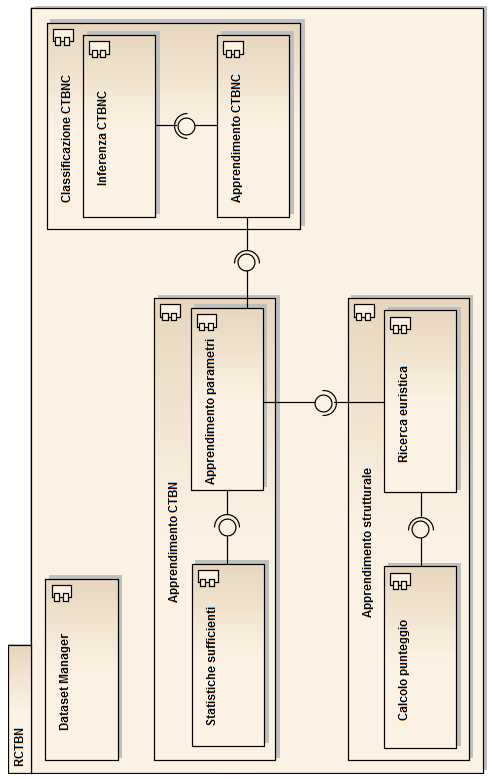
\includegraphics[width=1\columnwidth]{rctbn-arch.png}
	\caption[Diagramma dei componenti di \rctbn{}]{Diagramma dei componenti di \rctbn{}.}
	\label{fig:rctbncomponents}
\end{figure}


%\omissis{}


%\omissis{}

%scopo
%vincoli: da chi deve essere usato? dove deve essere installato? attori? -> casi d'uso (con precondinzioni)
%requisiti: il sistema deve permettere ..
%tabella casi d'uso/requisiti?

%\section{Package CTBN}
%\omissis{}

%\subsection{Gestione dei dati}\label{subsec:rctbn-ds-management}
%\omissis{}

%\subsection{Apprendimento}\label{subsec:rctbn-learning}
%\omissis{}

%\subsection{Inferenza}\label{subsec:rctbn-inference}
%\omissis{}

%\subsection{Apprendimento strutturale}\label{subsec:rctbn-structurallearning}
%\omissis{}

%\subsection{Package xvalidation}\label{subsec:rctbn-xvalidation}
%\omissis{}

% introdurre R? Rcpp?
% introdurre paradigma funzionale?
% architettura/componenti
% signature + documentazione funzioni principali?
% parlare dei task che supportano la parallelizzazione
% struttura package R
% componente cross-validation: spiegare metriche di valutazione utilizzate? si! ma in capitolo 4!
